%-------------------------------------------------------------------------------
% Special Cosserat rods
%-------------------------------------------------------------------------------
\section{Theory of Special Cosserat rods}

%-------------------------------------------------------------------------------
\begin{frame}
  \frametitle{Introduction to \st{special} Cosserat rods (part 1)}
  \vspace{-1em}
  \begin{figure}
    \centering
    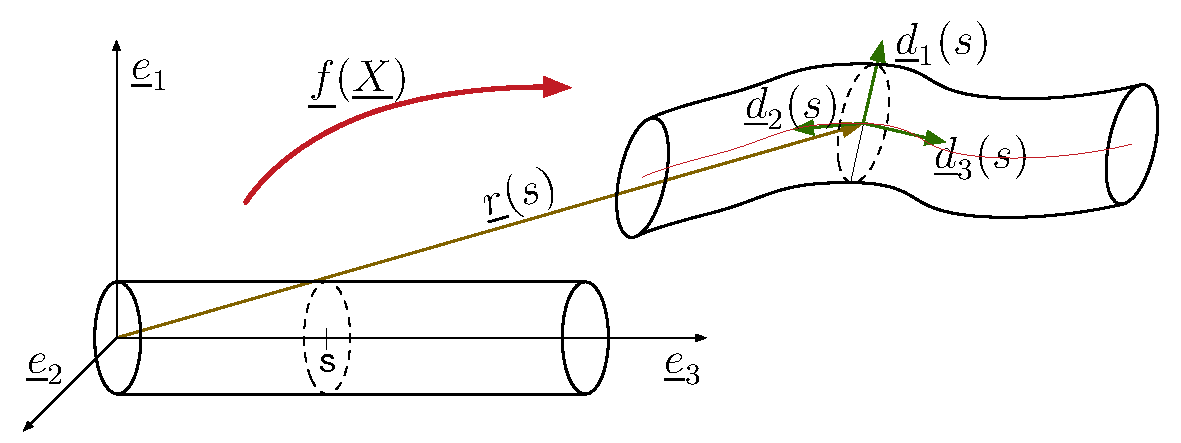
\includegraphics[width=20cm, keepaspectratio=true]{sections/cosserat_rods/images/Kinematics}
  \end{figure}
  
  Remember: $s$ is the unique identifier for a particular cross section of the beam
  \vspace{0.6em}
  
  Kinematic quantities:
  \begin{itemize}
    \item position of the deformed cross section $\underline{r}(s)$
    \item shearing of the deformed cross section $\underline{d}_1(s)$, $\underline{d}_2(s)$
    \item orientation of the deformed cross section $\underline{d}_3(s)$ \newline
      \null \quad (perpendicular to $\underline{d}_1(s)$ and $\underline{d}_2(s)$ $\rightarrow$ not independent)
    %\item $\doubleunderline{R}(s)$
  \end{itemize}
  
\end{frame}


%-------------------------------------------------------------------------------
\begin{frame}
  \frametitle{Introduction to \st{special} Cosserat rods (part 2)}

  Constrained deformation map:
  \begin{displaymath}
    \underline{f}(\underline{X}) = \underline{f}(X_1,X_2,X_3=s) = \underline{r}(s) + X_{\alpha} \, \underline{d}_{\alpha} \quad \text{with } \alpha \in \{1,2\}
  \end{displaymath}
  
  Consequences:
  \begin{itemize}
    \item cross sections remain flat
    \item straight lines within the cross section remain straight lines
    \item boundary of the cross section: circles are mapped to ellipses \newline
      \null \quad (not to arbitrary  curves in 2D)
    \item $\underline{d}_1(s)$ and $\underline{d}_2(s)$ are not perpendicular in the general case (shearing)
  \end{itemize}

\end{frame}



%-------------------------------------------------------------------------------
\begin{frame}
  \frametitle{Kinematics of the Special Cosserat rod}

  What makes the Special Cosserat rod special?:
  \begin{itemize}
    \item $\underline{d}_1(s)$ and $\underline{d}_2(s)$ \textit{are} perpendicular and unit-normed
    \item hence $\left( \underline{d}_1, \underline{d}_2, \underline{d}_3 \right)$ form an orthonormal triad
  \end{itemize}
  \vspace{0.6em}
  
  Consequences:
  \begin{displaymath}
    \exists \: \doubleunderline{R}(s) \in SO3 \: \forall s : \biggl( R: \left( \underline{e}_1, \underline{e}_2, \underline{e}_3 \right) \mapsto \left( \underline{d}_1, \underline{d}_2, \underline{d}_3 \right) \biggr)
  \end{displaymath}
  % TODO SO3 (twice)
  \begin{itemize}
    \item $\left( \underline{e}_1, \underline{e}_2, \underline{e}_3 \right)$ is called the global basis
    \item $\left( \underline{d}_1, \underline{d}_2, \underline{d}_3 \right)(s)$ is called the local basis or director basis at $s$
    \item $\underline{d}_i(s) = \doubleunderline{R}(s) \cdot \underline{e}_i$ \quad 
      ($\doubleunderline{R}$ : rotation matrix ; $SO3$ : special orthogonal matrix group)
  \end{itemize}
  \vspace{0.6em}
  
  Constrained deformation map:
  \begin{displaymath}
    \underline{f}(\underline{X}) = \underline{f}(X_1,X_2,X_3=s) = \underline{r}(s) + \doubleunderline{R}(s) \cdot (X_{\alpha} \, \underline{e}_{\alpha}) \quad \text{with } \alpha \in \{1,2\}
  \end{displaymath}
  
  \vspace{0.5em}
  Remark: The rigidity of the cross section is stiffening the beam!
\end{frame}


%-------------------------------------------------------------------------------
\begin{frame}
  \frametitle{Kinematics of the Special Cosserat rod (warp-mode on ;-)}
  
  MESSED UP:
  Remember: more accuracy $\rightarrow$ more unknowns
  \vspace{0.6em}
  % TODO check again from here , extra unknown
  We introduce warping of the cross section, 
  while at the same time keeping the director basis $\underline{d}_i$. Modified deformation map:
  \begin{displaymath}
    \underline{f}(\underline{X}) = \underline{f}(X_1,X_2,X_3=s) = \underline{r}(s) + \doubleunderline{R}(s) \cdot (X_{\alpha} \, \underline{e}_{\alpha} + \underline{u}) \quad \text{with } \alpha \in \{1,2\}
  \end{displaymath}
  
  in-plane: shrinking
  out-of-plane: warping, not planar
  
  if $\underline{u}(X_1,X_2)$ then we would again deal with a 3D elasticity problem \newline
  % small x?
  $\rightarrow$ $\underline{u}$ depends on local measures (1D theory)
  $\underline{u}$ is not an independent quantity / extra unknown
  
  $\underline{u}(X_1,X_2,\text{local strains})$
  local strains: local gradients of $\underline{r}$ and $\doubleunderline{R}$
  
  $\underline{d}_1$, $\underline{d}_1$ are perpendicular and represent the average orientation of the warped cross section
  
\end{frame}



%-------------------------------------------------------------------------------
\begin{frame}
  \frametitle{...}
  
  % TODO order of slides
  3D elasticity , plug in the constrained deformation map , integrate over cross section , obtain a system of ODEs in the unknowns $\underline{r}(s)$ and $\doubleunderline{R}(s)$
  
\end{frame}

%-------------------------------------------------------------------------------
\begin{frame}
  \frametitle{Rotations in 3D revisited}
  
  A rotation about \textit{one} axis is determined by
  \begin{itemize}
    \item axis of rotation given by $\underline{a}$ with $\norm{\underline{a}} = 1$
    \item angle of rotation $\Theta$
  \end{itemize}
  \vspace{0.6em}
  
  Composition of rotations:
  \begin{displaymath}
    \left( \underline{a}_1, \Theta_1 \right) + \left( \underline{a}_2, \Theta_2 \right) + \left( \underline{a}_3, \Theta_3 \right) + \dots = \left( \underline{a}_{eff}, \Theta_{eff} \right)
  \end{displaymath}
  \begin{displaymath}
    \doubleunderline{R}_{eff} = \dots \cdot \doubleunderline{R}_3 \cdot \doubleunderline{R}_2 \cdot \doubleunderline{R}_1
  \end{displaymath}
  Remark: In the general case ($\underline{a}_i \neq \underline{a}_j \text{ for } i \neq j$) rotations do not commute!
  \vspace{1em}
  
  Example (rotation about $\underline{e}_3$):
  \begin{displaymath}
    \Biggl( \underline{a} =
    \begin{bmatrix}
      0 \\ 0 \\ 1
    \end{bmatrix}, \Theta \Biggr) \quad \rightarrow \quad
    \doubleunderline{R} =
    \begin{bmatrix}
      +\cos(\Theta) & -\sin(\Theta) & 0 \\
      +\sin(\Theta) & +\cos(\Theta) & 0 \\
      0 & 0 & 1
    \end{bmatrix}
  \end{displaymath}

\end{frame}

%-------------------------------------------------------------------------------
\begin{frame}
  \frametitle{Axis-angle representation of rotations in 3D}
  
  From the axis-angle representation
  \begin{displaymath}
    \Biggl( \underline{a} =
    \begin{bmatrix}
      a_1 \\ a_2 \\ a_3
    \end{bmatrix}, \Theta \Biggr)
  \end{displaymath}
  we obtain the corresponding rotation matrix
  \begin{displaymath}
    \doubleunderline{R} = \exp(\Theta \cdot \doubleunderline{a})  
  \end{displaymath}
  with
  \begin{displaymath}
    \Theta \cdot \doubleunderline{a} = \Theta \cdot 
    \begin{bmatrix}
      0 & -a_3 & a_2 \\
      a_3 & 0 & -a_1 \\
      -a_2 & a_1 & 0
    \end{bmatrix}
  \end{displaymath}
  a skew-symmetric matrix obtained from the definition $\doubleunderline{a} = \doubleunderline{a} \cdot \doubleunderline{I} = \underline{a} \times \doubleunderline{I}$
  
  \vspace{2em}
  Observe the isomorphism between cross products and skew-symmetric matrices:
  \begin{displaymath}
    \underline{a} = \axial(\doubleunderline{a}) = \axial(\underline{a} \times \doubleunderline{I}) = \axial([\underline{a}]_{\times})
  \end{displaymath}
\end{frame}


%-------------------------------------------------------------------------------
\begin{frame}
  \frametitle{Axis-angle representation of rotations in 3D: Rodrigues' formula}
  
  The Rodrigues' rotation formula allows us to compute the rotation matrix $\doubleunderline{R}$ that corresponds to a given axis-angle representation $\left( \underline{a}, \Theta \right)$ without actually computing the matrix exponential
  
  \begin{displaymath}
    \doubleunderline{R} = \cos(\Theta) \, \doubleunderline{I} + \sin(\Theta) \, \doubleunderline{a} + (1-\cos(\Theta)) \, \underline{a} \otimes \underline{a}
  \end{displaymath}
  
  Example:
  \begin{displaymath}
    \underline{v}_{\text{rotated}} = \doubleunderline{R} \, \underline{v} = \cos(\Theta) \, \underline{v} + \sin(\Theta) \underline{a} \times \underline{v} + (1-\cos(\Theta)) \, (\underline{a} \cdot \underline{v}) \,\underline{a}
  \end{displaymath}
  
%  \begin{displaymath}
%    \doubleunderline{R} = \exp([\underline{a}]_{\times}) = \doubleunderline{I} + \sin(\norm{\underline{a}}) \biggl( \frac{\underline{a}}{\norm{\underline{a}}} \biggr)
%  \end{displaymath}

\end{frame}


%-------------------------------------------------------------------------------
\begin{frame}
  \frametitle{3D rotations expressed by unit quaternions}
  
  Quaternions are a number system that extends the complex numbers. A quaternion consists of one real part and three independent imaginary parts. A unit quaternion is a quaternion of norm one and therefore has three independent components. There exists an isomorphism between unit quaternions and rotation matrices
  % TODO check if formulas are valid? more info on this stuff useful?
  \begin{displaymath}
    \text{given }
    \underline{q} = \begin{bmatrix}
      q_0 \\ q_1 \\ q_2 \\ q_3
    \end{bmatrix} \quad \rightarrow \quad
    \doubleunderline{R}(\underline{q}) = 2 \cdot \begin{bmatrix}
      \frac{1}{2} - (q_2^2 + q_3^2) & q_1 \, q_2 - q_0 \, q_3 & q_1 \, q_3 + q_0 \, q_2 \\
      q_1 \, q_2 + q_0 \, q_3 & \frac{1}{2} - (q_1^2 + q_3^2) & q_2 \, q_3 - q_0 \, q_1 \\
      q_1 \, q_3 - q_0 \, q_2 & q_2 \, q_3 + q_0 \, q_1 & \frac{1}{2} - (q_1^2 + q_2^2)
    \end{bmatrix}
  \end{displaymath}
  
  \begin{displaymath}
    \text{real part: } q_0 = \cos \biggl( \frac{\Theta}{2} \biggr) \: \text{ and imaginary part: } \begin{bmatrix}
      q_1 \\ q_2 \\ q_3
    \end{bmatrix} = \sin \biggl( \frac{\Theta}{2} \biggr) \, \underline{a}
  \end{displaymath}
  
  advantage: quadratic polynomials are much faster for computation than $\sin(.)$ and $\cos(.)$

\end{frame}



